\documentclass[10pt,twocolumn]{ctexart}
\usepackage{morelull}
\usepackage{enumerate}
\usepackage{bm}
\usepackage{makecell}
\usepackage{xcolor}
\usepackage{graphicx}
\usepackage{subfigure}
\usepackage{framed}%包中有添加文字背景色命令shaded
\colorlet{shadecolor}{MaterialBlue50}
\usepackage{tabularx}
\usepackage{multicol}
\setlength{\columnsep}{12pt}
\setlength{\columnseprule}{1pt}
\usepackage{flushend,cuted}
\usepackage{multirow}
\usepackage{indentfirst}
\usepackage{amsmath,amssymb,amsthm,bm,bbding,pifont,dsfont}
\usepackage{mathtools}
\newcommand{\abs}[1]{\left| #1 \right|}
\usepackage{caption}
\captionsetup[figure]{labelfont={bf},labelformat={default},labelsep=period,name={图}}
%定义选择题选项
\newcommand{\onech}[4]{
\renewcommand\arraystretch{1.4}
\begin{tabularx}{\linewidth}{XXXX}
\setlength\tabcolsep{0pt}
(A) #1 & (B) #2 & (C) #3 & (D) #4 \\
\end{tabularx}
\unskip \unskip}
\newcommand{\twoch}[4]{
\renewcommand\arraystretch{1.4}
\begin{tabularx}{\linewidth}{XX}
\setlength\tabcolsep{0pt}
(A) #1 & (B) #2 \\
(C) #3 & (D) #4
\end{tabularx}
\unskip \unskip}

\title{初中数学必学的数学模型}
\author{安徽省霍邱县龙潭中心校}
\date{\today}



\begin{document}

\maketitle
\tableofcontents


\clearpage
\begin{strip}
\section{角的飞镖模型和“8”字模型}
\subsection{角的飞镖模型}

\begin{custom}[explorecolor]{飞镖模型}
\begin{minipage}{0.3\textwidth}
 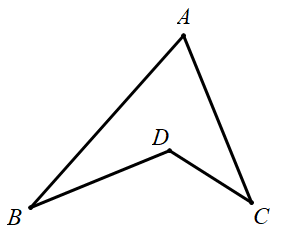
\includegraphics[scale=0.3]{figure/feibiao01.PNG}
\end{minipage}
\begin{minipage}{0.6\textwidth}
结论\ding{192}:\textcolor{red}{$\angle BDC=\angle A+\angle B+\angle C$}\\
结论\ding{193}:\textcolor{red}{$AB+AC>BD+CD$}
\end{minipage}
\end{custom}
\end{strip}







对于结论\ding{193}的证明,主要利用\textcolor{red}{三角形两边之和大于第三边}进行证明.

\begin{minipage}{0.6\textwidth}

\kaishu\color{cyan}{证明:延长$BD$,交$AC$于点$E$,如图.\\
$\because AB+AE>BE, CE+DE>CD\\ 
\therefore AB+AE+CE+DE>BE+CD\\
\therefore AB+AC+DE>BD+DE+CD\\
\therefore AB+AC>BD+CD$}
\end{minipage}
\begin{minipage}{0.4\textwidth}
 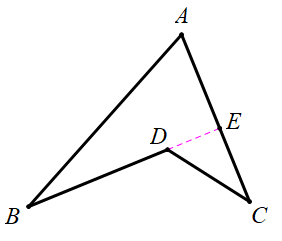
\includegraphics[scale=0.5]{figure/feibiao02.PNG}
\end{minipage}

\subsubsection{飞镖模型例题}
\begin{example}
如图,在四边形$ABCD$中,$AM$、$CM$分别平分$\angle DAB$和$\angle DCB$,$AM$与$CM$交于点$M$,探究$\angle AMC$与$\angle B$、$\angle D$之间的数量关系.
\end{example}
 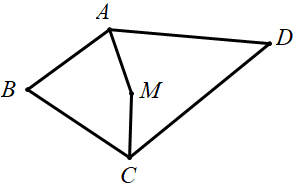
\includegraphics[scale=0.5]{figure/feibiao04.PNG}
 
\begin{example}
如图,已知$\angle DEC=100^\circ$,$\angle CFB=120^\circ$,求$\angle A+\angle B+\angle C+\angle D=$\underline{~\hspace{1cm}~}
\end{example}

 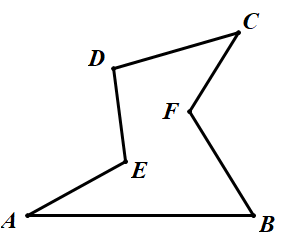
\includegraphics[scale=0.5]{figure/feibiao05.PNG}

\begin{example}
如图,求$\angle A+\angle B+\angle C+\angle D+\angle E+\angle F=$\underline{~\hspace{1cm}~}
\end{example}

 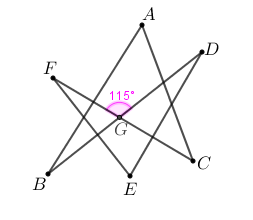
\includegraphics[scale=0.5]{figure/feibiao06.PNG}

\begin{example}
如图,在$\triangle ABC$中,$\angle A=52^\circ$,$\angle ABC$与$\angle ACB$的角平分线交于点$D_1$,$\angle ABD_1$与$\angle ACD_1$的角平分线交于点$D_2$,以此类推,$\angle ABD_4$与$\angle ACD_4$的角平分线交于点$D_5$,则$\angle BD_5C$是\underline{~\hspace{1cm}~}度.
\end{example}

 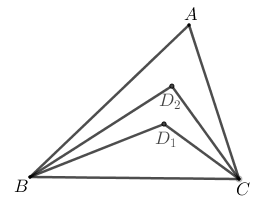
\includegraphics[scale=0.6]{figure/feibiao07.PNG}

\begin{example}
如图1,在$\triangle ABC$中,$\angle ABC,\angle ACB$的角平分线交于点$O$,则$\angle BOC=90^\circ+\dfrac{1}{2}\angle A=\dfrac{1}{2}\times 180^\circ+\dfrac{1}{2}\angle A$.如图2和图3,在$\triangle ABC$中,$\angle ABC,\angle ACB$的两条三等分角线分别对应交于$O_1,O_2$,则$\angle BO_1C=\dfrac{2}{3}\times 180^\circ+\dfrac{1}{3}\angle A,\angle BO_2C=\dfrac{1}{3}\times 180^\circ+\dfrac{2}{3}\angle A$.根据以上阅读理解,你能猜想$\angle BO_{2020}C$\underline{~\hspace{1cm}~}
\end{example}

 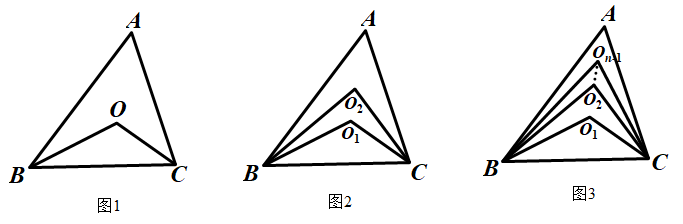
\includegraphics[scale=0.6]{figure/feibiao08.PNG}


\subsection{“8”字模型}

\begin{custom}[explorecolor]{“8”字模型}
\begin{minipage}{0.3\textwidth}
 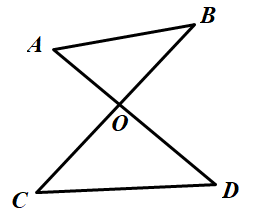
\includegraphics[scale=0.3]{figure/bazhi01.PNG}
\end{minipage}
\begin{minipage}{0.6\textwidth}
如图,线段$AD,BC$相交于点$O$,连接$AB,CD$.\\
结论\ding{192}:\textcolor{red}{$\angle A+\angle B=\angle C+\angle D$}\\
结论\ding{193}:\textcolor{red}{$AB+CD>AD+BC$}
\end{minipage}
\end{custom}
下面对结论\ding{192}进行证明,分别根据\textcolor{red}{三角形内角和等于$180^\circ$}及\textcolor{red}{三角形外角的性质}有两种证法,如下:

\begin{minipage}{0.5\textwidth}
\kaishu\color{cyan}{证法\ding{192}:利用三角形内角和等于180\\
$\angle A+\angle B+\angle AOB=180^\circ,\\
\angle C+\angle D+\angle COD=180^\circ\\
\therefore \angle A+\angle B+\angle AOB=\angle C+\angle D+\angle COD\\
\because \angle AOB=\angle COD\\
\therefore \angle A+\angle B=\angle C+\angle D.$}
\end{minipage}
\begin{minipage}{0.5\textwidth}
\kaishu\color{cyan}{证法\ding{193}:利用三角形外角的性质\\
$\because \angle BOD=\angle A+\angle B\\
\angle BOD=\angle C+\angle D\\
\therefore \angle A+\angle B=\angle C+\angle D.$}
\end{minipage}
\subsubsection{“8”字模型例题}
\begin{shaded}
\begin{example}
如图,求$\angle A+\angle B+\angle C+\angle D+\angle E=$\underline{~\hspace{1cm}~}.
\end{example}
\end{shaded}
 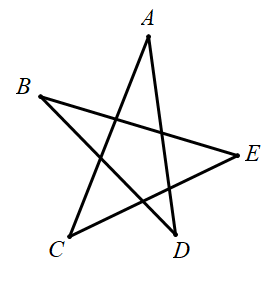
\includegraphics[scale=0.5]{figure/bazhi02.PNG}
\begin{shaded}
\begin{example}
如图,则$\angle A+\angle B+\angle C+\angle D+\angle E$的度数为\underline{~\hspace{1cm}~}.
\end{example}
\end{shaded}
 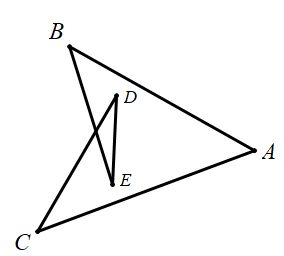
\includegraphics[scale=0.5]{figure/bazhi03.PNG}
\begin{shaded}
\begin{example}
如图,$\angle A+\angle B+\angle C+\angle D+\angle E=$\underline{~\hspace{1cm}~}.
\end{example}
\end{shaded}
 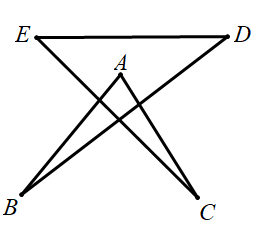
\includegraphics[scale=0.5]{figure/bazhi04.PNG}
\begin{shaded}
\begin{example}
如图,则$\angle A+\angle B+\angle C+\angle D+\angle E+\angle F=(~\hspace{1cm}~)$\\
\onech{$180^\circ$}{$360^\circ$}{$270^\circ$}{$540^\circ$}
\end{example}
\end{shaded}
 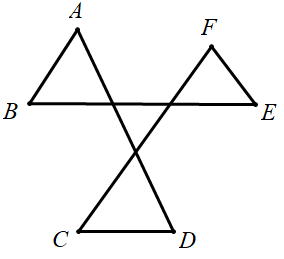
\includegraphics[scale=0.5]{figure/bazhi05.PNG}
\begin{shaded}
\begin{example}
如图,则$\angle A+\angle B+\angle C+\angle D+\angle E+\angle G+\angle H$的度数为\underline{~\hspace{1cm}~}.
\end{example}
\end{shaded}
 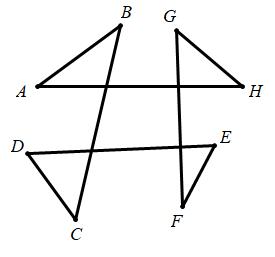
\includegraphics[scale=0.5]{figure/bazhi06.PNG}
\begin{shaded}
\begin{example}
如图,则$\angle A+\angle B+\angle C+\angle D+\angle E+\angle G+\angle H=$\underline{~\hspace{1cm}~}.
\end{example}
\end{shaded}
 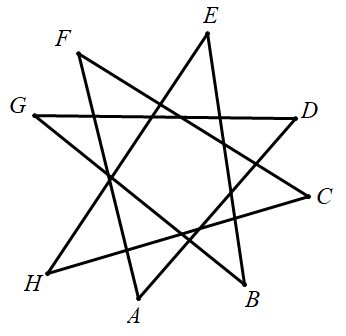
\includegraphics[scale=0.5]{figure/bazhi07.PNG}
\begin{shaded}
\begin{example}
如图,则$\angle A+\angle B+\angle C+\angle D+\angle E+\angle G+\angle H+\angle I+\angle K$的度数为$(~\hspace{1cm}~)$.\\
\onech{$720^\circ$}{$900^\circ$}{$1080^\circ$}{$1260^\circ$}
\end{example}
\end{shaded}
 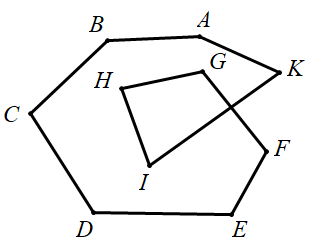
\includegraphics[scale=0.5]{figure/bazhi08.PNG}
\subsection{飞镖模型和“8”字模型进阶练习}

1.如图,$\angle A+\angle B+\angle C+\angle D+\angle E$的度数是\underline{~\hspace{1cm}~}.

 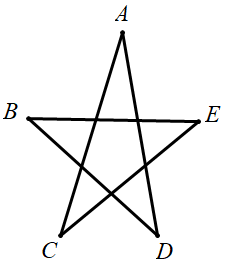
\includegraphics[scale=0.5]{figure/bazhi09.PNG}
 
2.如图,$\angle A+\angle B+\angle C+\angle D+\angle E=$\underline{~\hspace{1cm}~}.

 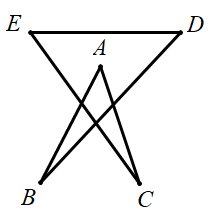
\includegraphics[scale=0.5]{figure/bazhi10.PNG}
 
3.如图,若$\angle A+\angle B+\angle C+\angle D+\angle E+\angle F=660^\circ$,求$\angle G+\angle H$的度数.

 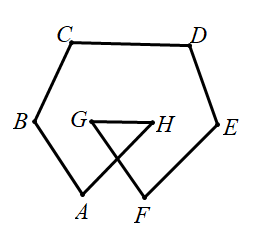
\includegraphics[scale=0.5]{figure/bazhi11.PNG}
 
4.如图,求$\angle A+\angle B+\angle C+\angle D+\angle E+\angle F+\angle G+\angle H+\angle K$的度数.

 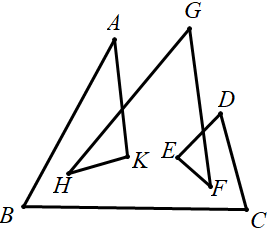
\includegraphics[scale=0.5]{figure/bazhi12.PNG}
 
5.如图,求$\angle A+\angle B+\angle C+\angle D+\angle E+\angle F$的度数.

 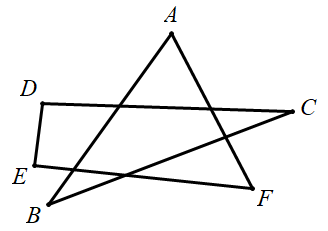
\includegraphics[scale=0.5]{figure/bazhi15.PNG}
 
6. (1)如图\ding{192},求$\angle A+\angle B+\angle C+\angle D+\angle E+\angle F$的度数.\\
    (2)如图\ding{193},求$\angle A+\angle B+\angle C+\angle D+\angle E+\angle F+\angle G+\angle H$的度数.\\
    (3)如图\ding{194},求$\angle A+\angle B+\angle C+\angle D+\angle E+\angle F+\angle G$的度数.
    
 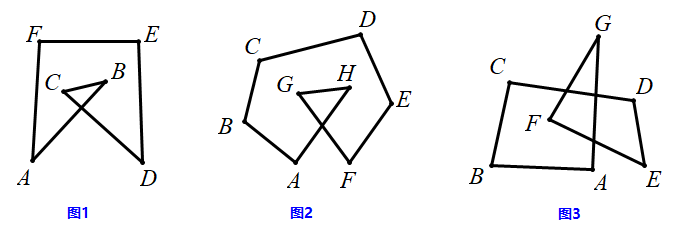
\includegraphics[scale=0.5]{figure/bazhi13.PNG}
 
7.如图,$BE$与$CD$相交于点$A$,$CF$为$\angle BCD$的平分线,$EF$为$\angle BED$的角平分线,若$\angle B:\angle D:\angle F=2:4:x$,求$x$的值.

 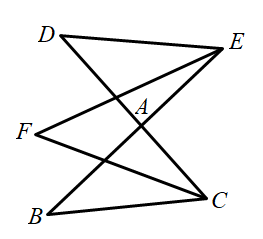
\includegraphics[scale=0.5]{figure/bazhi14.PNG}

\section{手拉手模型——旋转全等}
\subsection{手拉手模型的定义及基本结论}
\begin{custom}[explorecolor]{手拉手全等模型}
所谓手拉手模型,是指\textcolor{red}{顶角相等},且有\textcolor{red}{公共顶点}的两个\textcolor{red}{等腰三角形}组成的图形,从中可以得到一个经典的全等模型:因为顶点相连的四条边,形象的可以看作两双手,所以通常称为“手拉手模型”.

\begin{minipage}{0.3\textwidth}
 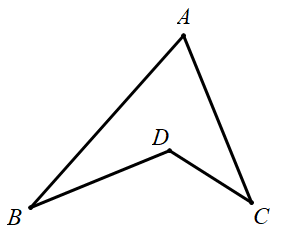
\includegraphics[scale=0.3]{figure/feibiao01.PNG}
\end{minipage}
\begin{minipage}{0.6\textwidth}
结论\ding{192}:\textcolor{red}{$\angle BDC=\angle A+\angle B+\angle C$}\\
结论\ding{193}:\textcolor{red}{$AB+AC>BD+CD$}
\end{minipage}
\end{custom}

\subsection{手拉手模型的常见类型}
\section{半角模型}
\section{十字架模型}
\section{三垂直全等模型}
\section{角平分线模型}
\section{胡不归}
\section{阿氏圆}
\section{倍长中线}
\section{对角互补}






\end{document}